\documentclass{ximera}

\input{../preamble.tex}

\title[Dig-In:]{Parametric surfaces}

\begin{document}
\begin{abstract}
  Tangent and normal vectors can help model surfaces in space.
\end{abstract}
\maketitle

Unit tangent vectors and unit normal vectors can help us to model
surfaces in space.

\section{Thickening a curve}

Suppose you have been a curve in space, and you want to build a
parameterized surface which is a ``thickened'' version.  In other
words, we want to convert a curve like
\begin{image}
  \includegraphics{curve.jpg}
\end{image}
%% \begin{sageOutput}
%% x(t) = sin(t)
%% y(t) = sin(2*t + pi/5)
%% z(t) = sin(3*t + pi/7)
%% f(t) = (x(t),y(t),z(t))
%% parametric_plot3d(f(t), (t,0,2*pi))
%%   \end{sageOutput}
into a thickened ``tube'' like
\begin{image}
  \includegraphics{tube.jpg}
\end{image}
%% \begin{sageOutput}
%% var('s')
%% x(t) = sin(t)
%% y(t) = sin(2*t + pi/5)
%% z(t) = sin(3*t + pi/7)
%% f(t) = (x(t),y(t),z(t))
%% df=derivative(f,t)
%% ut = df / df.norm()
%% ddf = derivative(ut,t)
%% n = ddf / ddf.norm()
%% bn = n.cross_product(ut)
%% thickness = 0.10
%% parametric_plot3d(f(t) + (n * cos(s) + bn * sin(s)) * thickness, (t,0,2*pi), (s,0,2*pi), plot_points=[100,100])
%%   \end{sageOutput}
  
\begin{image}
  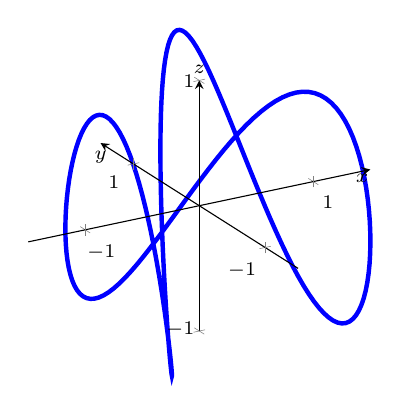
\begin{tikzpicture}
    \begin{axis}[tick label style={font=\scriptsize},axis on top,view={-30}{30},no markers,zmax=1,axis lines=center,
        ymax=1.5,ymin=-1.5,clip=false,
        xmax=1.5,xmin=-1.5,
        every axis x label/.style={at={(axis cs:\pgfkeysvalueof{/pgfplots/xmax},0,0)},xshift=-3pt,yshift=-3pt},
	xlabel={\scriptsize $x$},
	every axis y label/.style={at={(axis cs:0,\pgfkeysvalueof{/pgfplots/ymax},0)},xshift=0pt,yshift=-5pt},
	ylabel={\scriptsize $y$},
	every axis z label/.style={at={(axis cs:0,0,\pgfkeysvalueof{/pgfplots/zmax})},xshift=0pt,yshift=4pt},
	zlabel={\scriptsize $z$}]
      \addplot3+[domain=-0:360,samples=200,samples y=0,ultra thick](sin(x),{sin(2*x+36},{sin(3*x+25)});
    \end{axis}
  \end{tikzpicture}
\end{image}

\begin{example}[Thickening a curve]
  You have been given a curve in space, meaning that you have been
  given a function
  \begin{multipleChoice}
    \choice{$f: \R \to \R$}
    \choice{$F: \R^3 \to \R$}
    \choice[correct]{$\vec{f}: \R \to \R^3$}
  \end{multipleChoice}
  and your task is to build a parameterized surface which is a
  ``thickened'' version.
  
  In other words, we want to convert a curve like
  \begin{sageCell}
x(t) = sin(t)
y(t) = sin(2*t + pi/5)
z(t) = sin(3*t + pi/7)
f(t) = (x(t),y(t),z(t))
parametric_plot3d(f(t), (t,0,2*pi))
  \end{sageCell}
  into a thickened ``tube'' like
  \begin{sageOutput}
x(t) = sin(t)
y(t) = sin(2*t + pi/5)
z(t) = sin(3*t + pi/7)
f(t) = (x(t),y(t),z(t))
df=derivative(f,t)
ut = df / df.norm()
ddf = derivative(ut,t)
n = ddf / ddf.norm()
bn = n.cross_product(ut)
thickness = 0.10
parametric_plot3d(f(t) + (n * cos(s) + bn * sin(s)) * thickness, (t,0,2*pi), (s,0,2*pi), plot_points=[100,100])
  \end{sageOutput}

  Our tube around $\vec{f}$ will be a parametrized surface given by 
  \begin{multipleChoice}
    \choice{$\vec{f}: \R \to \R^2$}
    \choice{$F: \R^2 \to \R$}
    \choice[correct]{$\vec{F}: \R^2 \to \R^3$}
    \choice{$\vec{F}: \R^3 \to \R^2$}
  \end{multipleChoice}

  We can parametrize a circle with
  \begin{multipleChoice}
    \choice{$t \mapsto (x^2, y^2)$}
    \choice{$t \mapsto (\cos^2(t), \sin^2(t))$}
    \choice[correct]{$t \mapsto (\cos(t), \sin(t))$}
  \end{multipleChoice}
  so we \textit{could} try
  \[
    \vec{F}(t,s) = \vec{f}(t) + 0.25 \vector{\cos s, \sin s, 0}.
  \]
  Note that we are using \textbf{vector operations}---we are taking the
\wordChoice{\choice[correct]{sum}\choice{dot product}} of two vectors to build up our parametrized surface.  We want the vector $\vec{f}(t)$ to sit \wordChoice{\choice{on the surface}\choice[correct]{inside the tube}} and the second term pushes us away from $\vec{f}(t)$ in a different direction as $s$ varies.  The factor of 0.25 is included to \wordChoice{\choice[correct]{shrink the circle}\choice{expand the circle}}.  Putting this together, we can see a picture emerging:
  \begin{sageCell}
t = var('t')
x = sin(t) ; y = sin(2*t + pi/5) ; z = sin(3*t + pi/7)
f = vector([x,y,z])

s = var('s')
parametric_plot3d( f + 0.25 * vector([cos(s), sin(s), 0]), (t,0,2*pi), (s,0,2*pi) )
\end{sageCell}
and that doesn't look awful, but it also certainly doesn't quite look
right!  The trouble is the circle we sweep out with
$\vector{\cos s, \sin s, 0}$ is not always
\wordChoice{\choice[correct]{perpendicular}\choice{parallel}} to the
unit tangent vector, defined as
\begin{multipleChoice}
  \choice{$\utan(t) = \frac{\vec{f}'(t)}{|\vec{f}'(t)|^2}$}
  \choice[correct]{$\utan(t) = \frac{\vec{f}'(t)}{|\vec{f}'(t)|}$}
\end{multipleChoice}
To improve our tube, we want to sweep out a circle in the plane given by
\begin{multipleChoice}
  \choice{$\utan(t)$ and $\unormal(t)$}
  \choice{$\utan(t)$ and $\unormal(t) \cross \utan(t)$}
  \choice[correct]{$\unormal(t)$ and $\unormal(t) \cross \utan(t)$}
\end{multipleChoice}
Let $\vec{b} = \unormal(t) \cross \utan(t)$ and $\ubinormal = \frac{\vec{b}}{| \vec{b} |}$.  Then we can sweep out a tube with
  \[
    \vec{F}(t,s) = \vec{f}(t) + 0.25 \left( \left( \cos \answer{s} \right) \unormal(\answer{t}) + \left( \sin s \right) \ubinormal(t) \right)
  \]
  to keep our circle in the appropriate plane.  Try it!
\begin{sageCell}
t = var('t')
x = sin(t) ; y = sin(2*t + pi/5) ; z = sin(3*t + pi/7)

f = vector([x,y,z])
df = derivative(f,t)
u = df.normalized()
n = derivative(u,t).normalized()
b = n.cross_product(u).normalized()

thickness = 0.25
s = var('s')
parametric_plot3d( f + (n * cos(s) + b * sin(s)) * thickness, (t,0,2*pi), (s,0,2*pi), plot_points=[100,100] )
\end{sageCell}
\end{example}  

\begin{example}[Mirrored surfaces]
  We have a parametrized surface 
  \begin{multipleChoice}
    \choice{$\vec{f}: \R \to \R^2$}
    \choice{$F: \R^2 \to \R$}
    \choice[correct]{$\vec{F}: \R^2 \to \R^3$}
    \choice{$\vec{F}: \R^3 \to \R^2$}
  \end{multipleChoice}
  given by $(a,b) \mapsto (a, b, a^2 + b^2)$.  In this case, the surface is a 
  \begin{multipleChoice}
    \choice{sphere}
    \choice[correct]{paraboloid}
    \choice{hyperboloid}
  \end{multipleChoice}
  and we would like to understand how light would reflect off such an
  object, if we were to build it as a physical object.

  Suppose $\vec{\ell}(t)$ is an arbitrary (parametrized!) straight line, given by
  \begin{multipleChoice}
    \choice[correct]{$\vec{\ell}(t) = \vec{\ell}_0 + t \vec{v}$}
    \choice{$\vec{\ell}(t) = t \vec{\ell}_0 + t \vec{v}$}
    \choice{$\vec{\ell}(t) = \vec{\ell}_0 + \vec{v}$}
  \end{multipleChoice}
  and suppose the image of $\vec{\ell}(t)$ intersects the image of $\vec{F}$ at a point $(x,y,z)$.  

\begin{sageCell}
# The purple surface
a = var('a'); b = var('b')
f = vector([a,b,a^2 + b^2])

# The red light beam
t = var('t') ; ell0 = vector([0.85,0.5,1.5]) ; v = vector([-0.2,-0.1,-1])

parametric_plot3d( f, (a,-1,1), (b,-1,1) ) + parametric_plot3d( ell0 + t * v, (t,-0.5,2), color="red", thickness=0.1)
\end{sageCell}

When we zoom in close enough to the point $(x,y,z)$ where the light ray hits the surface, we imagine that the mirrored surface is \wordChoice{\choice[correct]{a plane}\choice{a line}} through the point $(x,y,z)$ and orthogonal to the vector
\begin{multipleChoice}
  \choice{$\pp{\vec{F}}{x} + \pp{\vec{F}}{y}$}
  \choice{$\pp{\vec{F}}{x} - \pp{\vec{F}}{y}$}
  \choice[correct]{$\pp{\vec{F}}{x} \cross \pp{\vec{F}}{y}$}
\end{multipleChoice}

When the light ray hits the surface, it is heading in the direction
\begin{multipleChoice}
  \choice{$\pp{\vec{F}}{x}$}
  \choice{$\pp{\vec{F}}{y}$}
  \choice[correct]{$\vec{v}$}
\end{multipleChoice}
This means that the reflected light will be heading in the direction
\begin{multipleChoice}
  \choice{$\vec{v} + 2 \proj_{\vec{v}} \pp{\vec{F}}{x} \cross \pp{\vec{F}}{y}$}
  \choice{$\vec{v} - 2 \proj_{\vec{v}} \pp{\vec{F}}{x} \cross \pp{\vec{F}}{y}$}
  \choice{$\vec{v} + 2 \proj_{\pp{\vec{F}}{x} \cross \pp{\vec{F}}{y}} \vec{v}$}
  \choice[correct]{$\vec{v} - 2 \proj_{\pp{\vec{F}}{x} \cross \pp{\vec{F}}{y}} \vec{v}$}
\end{multipleChoice}
Such formulas justify the time we spent thinking deeply about $\proj$.  And now we can plot all this together.
\begin{sageCell}
# The purple surface
a = var('a'); b = var('b')
f = vector([a,b,a^2 + b^2])

# The red light beam
t = var('t') ; ell0 = vector([0.85,0.5,1.5]) ; v = vector([0.1,-0.2,-1])

# The intersection of the surface and the light beam
solutions = solve( [f[i] == (ell0 + t*v)[i] for i in range(3)], [a,b,t], solution_dict=True)
solution = [s for s in solutions if t.subs(s) > 0][0]
xyz = f.subs(solution)

# The reflected vector
proj = lambda v, w: (v.dot_product(w))/(w.dot_product(w)) * w
n = derivative(f,a).cross_product( derivative(f,b) )
n = n.subs(solution)
rv = v - 2 * proj(v,n)

# Plot the surface, the incoming beam, and the outgoing beam
parametric_plot3d( f, (a,-1,1), (b,-1,1) ) + parametric_plot3d( ell0 + t * v, (t,-0.5,t.subs(solution)), color="red", thickness=0.1) + parametric_plot3d( xyz + t * rv, (t,0,2), color="red", thickness=0.1)
\end{sageCell}

\end{example}

\begin{example}[Vertical light]
  By playing around with the vector $\vec{v}$, i.e., the direction of
  the incoming light, we can discover some significant, qualitative
  features of reflections in paraboloids.

  Let $\vec{F}(x,y) = (x,y,x^2 + y^2)$, so that
  \begin{align*}
    \pp{\vec{F}}{x} &= \vector{ 1, 0, \answer{2x}} \\
    \pp{\vec{F}}{y} &= \vector{0, 1, \answer{2y}} \\
    \vec{n} &= \pp{\vec{F}}{x} \cross \pp{\vec{F}}{y} &= \vector{-2x, -2y, \answer{1}}. \\
  \end{align*}

  We want to focus in on the case of ``vertical light'' which arrives directly from above.  One way to 
  restrict to this situation would be to assume that both $\vec{v} \dotp \langle 1, 0, 0 \rangle = 0$ and
  $\vec{v} \dotp \vector{ 0, 1, 0 } = 0$, but to simplify the situation further, simply suppose
  that $\vec{v} = \vector{ 0, 0, -1 }$.  Then
  \begin{align*}
    \vec{v} - 2 \proj_{\vec{n}} (\vec{v}) 
    &= \vec{v} - 2 \frac{\vec{v} \dotp \vec{n}}{\vec{n} \dotp \vec{n}} \vec{n} \\
    &= \vec{v} - 2 \frac{\answer{-1}}{\vec{n} \dotp \vec{n}} \vec{n} \\
  \end{align*}
  This reflected vector simplies further to
  \[
    \frac{-4}{1 + 4x^2 + 4y^2} \vector{\answer{x}, \answer{y}, \answer{x^2 + y^2 - 1/4}}.
  \]
  The significance of this is that, starting at the point
  $(x,y,x^2 + y^2)$ and moving in the direction of this vector, we pass through the point 
  \[
    \left( 0, 0, \answer[given]{1/4} \right),
  \]
  meaning that \textit{every} vertical beam of light reflects off the
  paraboloid and is focused on common point!  This fact is what makes
  solar ovens and satellite dishes possible.
  
\end{example}




\end{document}
